%=================================================================================================
%= = = = = = = = = = = = = = = = = = = = = = = = = = = = = = = = = = = = = = = = = = = = = = = = =
%=																								 =
%=							   >  >  INFORMAÇÕES DO DOCUMENTO  <  <								 =
%=																								 =
%= = = = = = = = = = = = = = = = = = = = = = = = = = = = = = = = = = = = = = = = = = = = = = = = =
%=================================================================================================

\documentclass[a4paper,10pt,compsoc]{IEEEtran}

\usepackage{cmap}											%-> Mapear caracteres especiais no PDF
\usepackage[T1]{fontenc}									%-> Selecao de códigos de fonte
\usepackage[utf8]{inputenc}									%-> Codificacao do documento
\usepackage{indentfirst}									%-> Indenta o primeiro parágrafo seção
\usepackage{color}											%-> Controle das cores
\usepackage{graphicx}										%-> Inclusão de gráficos
\usepackage{units}											%-> 
\usepackage[english,brazil]{babel}							%-> documento em Português e Inglês
\usepackage{bold-extra}										%-> 
\usepackage{eso-pic}										%-> 
\usepackage{geometry}										%-> 


%=================================================================================================
%= = = = = = = = = = = = = = = = = = = = = = = = = = = = = = = = = = = = = = = = = = = = = = = = =
%=																								 =
%=									 CONFIGURAÇÕES DO HYPERREF									 =
%=																								 =
%= = = = = = = = = = = = = = = = = = = = = = = = = = = = = = = = = = = = = = = = = = = = = = = = =
%=================================================================================================


\setlength{\columnsep}{6mm}									%-> Distância entre as colunas
\geometry{left=1.5cm,right=1.5cm,top=1.5cm,bottom=1.5cm}	%-> 























%=================================================================================================
%= = = = = = = = = = = = = = = = = = = = = = = = = = = = = = = = = = = = = = = = = = = = = = = = =
%=================================================================================================									%-> Setup
%%=================================================================================================
%= = = = = = = = = = = = = = = = = = = = = = = = = = = = = = = = = = = = = = = = = = = = = = = = =
%=																								 =
%=									 	CRIAÇÃO DE COMANDOS										 =
%=																								 =
%= = = = = = = = = = = = = = = = = = = = = = = = = = = = = = = = = = = = = = = = = = = = = = = = =
%=================================================================================================


% - INSTRUÇÕES: -------------------------------------
% -													-
% - Este ambiente é destinado à criação de novos	-
% - comandos que conferirão a este documento		-
% - novas funcionalidades.							-
% -													-
% ---------------------------------------------------


% COMANDOS DE INFORMAÇÕES GERAIS DO DOCUMENTO ====================================================


% INFORMAÇÕES GERAIS -----------------------------------------------------------------------------

\newcommand{\citarautor}[1]{\def\imprimircitarautor{#1}}	%-> Comando para Citação de Autor

\newcommand{\instituto}[1]{\def\imprimirinstituto{#1}}		%-> Comando para Instituto

\newcommand{\faculdade}[1]{\def\imprimirfaculdade{#1}}		%-> Comando para Faculdade

\newcommand{\curso}[1]{\def\imprimircurso{#1}}				%-> Comando para Curso

\newcommand{\disciplina}[1]{\def\imprimirdisciplina{#1}}	%-> Comando para Grau Acadêmico


\newcommand{\local}[1]{\def\imprimirlocal{#1}}				%-> Comando para Grau Acadêmico

\newcommand{\data}[1]{\def\imprimirdata{#1}}				%-> Comando para Grau Acadêmico


% ORIENTADOR E COORIENTADOR - TITULAÇÃO ACADÊMICA ------------------------------------------------


%=================================================================================================
%= = = = = = = = = = = = = = = = = = = = = = = = = = = = = = = = = = = = = = = = = = = = = = = = =
%=================================================================================================								%-> Comandos para novas funcionalidades
%%=================================================================================================
%= = = = = = = = = = = = = = = = = = = = = = = = = = = = = = = = = = = = = = = = = = = = = = = = =
%=																								 =
%=							   >  >  INFORMAÇÕES DO DOCUMENTO  <  <								 =
%=																								 =
%= = = = = = = = = = = = = = = = = = = = = = = = = = = = = = = = = = = = = = = = = = = = = = = = =
%=================================================================================================


% - INSTRUÇÕES: -------------------------------------
% -													-
% - Preencha as informações gerais do documento	nos -
% - respectivos campos indicados.					-
% -													-
% ---------------------------------------------------



% TÍTULO =========================================================================================

\title{\textsf{
\bfseries \Huge Uso de Redes Neurais Artificiais na Previsão\\ 
do Consumo de Energia}}


% AUTORES =========================================================================================












%=================================================================================================
%= = = = = = = = = = = = = = = = = = = = = = = = = = = = = = = = = = = = = = = = = = = = = = = = =
%=================================================================================================							%-> Informações Gerais do Documento


\begin{document}

% ELEMENTOS PRÉ-TEXTUAIS =========================================================================

\twocolumn[
\begin{@twocolumnfalse}

\begin{center}
%=================================================================================================
%= = = = = = = = = = = = = = = = = = = = = = = = = = = = = = = = = = = = = = = = = = = = = = = = =
%=																								 =
%=							   		   >  >  CABEÇALHO  <  <									 =
%=																								 =
%= = = = = = = = = = = = = = = = = = = = = = = = = = = = = = = = = = = = = = = = = = = = = = = = =
%=================================================================================================


% - INSTRUÇÕES: -------------------------------------
% -													-
% - Preencha as informações gerais do documento	nos -
% - respectivos campos indicados.					-
% -													-
% ---------------------------------------------------


\begin{center}

% DADOS PESSOAIS =================================================================================

\vspace*{2 cm}

\textsf{\bfseries 
\huge Uso de Estruturas Competitiva de Redes Neurais \\[3 mm]
Auto Associativas na Classificação
de Tipos de Vinho}


% AUTORIA ========================================================================================

\vspace*{1.5 cm}

	\begin{large}
Luiz Henrique P. Assunção$^{1}$ e
Paulo Normando$^{2}$
	\end{large} \\[1.7 mm]


% DADOS DA INSTITUIÇÃO ===========================================================================

	\begin{small}
$^{1\ 2}$Faculdade de Engenharia Elétrica e Biomédica, Universidade Federal do Pará, \\[1 mm]
Av. Augusto Correa 01, Belém, Pará 66075-090, Brasil \\[7 mm]


% AUTORIA ========================================================================================

Autor Correspondente$^{1}$: luiz.heinrich@live.com	\\[1 mm]
Autor Correspondente$^{2}$: paulonormando@gmail.com

	\end{small}

\end{center}
 

%=================================================================================================
%= = = = = = = = = = = = = = = = = = = = = = = = = = = = = = = = = = = = = = = = = = = = = = = = =
%=================================================================================================			%->	Capa
%=================================================================================================
%=							       		      SUMÁRIO											 =
%=================================================================================================



\begin{center}


\begin{minipage}[c][5cm]{15cm}		%-> [Altura] [Largura]
	
\begin{abstract}

\noindent
O artigo detalha a construção e o uso de 2 estruturas de rede, ambas  aplicadas em um problema de classificação. A primeira estrutura baseia-se no modelo de rede Perceptron de múltiplas camadas(MLP), a outra estrutura é chamada de rede autoassociativa competitiva, também chamada de autoencoder competitiva. Essas estruturas foram aplicadas na classificação de tipos de vinho, visando-se assim comparar o desempenho e acurácia de ambas topologias no problema de classificação proposto.Ambas estruturas foram construídas utilizando software Python juntamente com a biblioteca Keras, o código utilizado na produção dos resultados está disponibilizado no github.  
\\[1 mm]
\textbf{Palavras-chave}: Redes Neurais Artificiais. Redes Auto Associativas. Vinho. MATLAB.

\end{abstract}

\end{minipage}


\end{center} \vspace*{0.5 cm}

					%->	Resumo
\end{center}

\end{@twocolumnfalse}]


% ELEMENTOS TEXTUAIS =============================================================================

%=================================================================================================
%=							       		    INTRODUÇÃO							     			 =
%=================================================================================================

\section{Introdução}
As Redes Neurais Artificiais (RNA) tratam-se de modelos matemáticos construídos a partir do conhecimento do neurônio biológico, tendo como objetivo mimetizar o comportamento da células nervosa \cite{ref1} . Assim, simulando a característica de um sistema nervoso, de forma a ter capacidade de processar múltiplas entradas, reconhecer e classificar padrões. Dessa forma, RNA tem grande capacidade de aplicação em vários tipos de contexto.

A aplicação proposta nesse artigo trata-se de classificação de tipos de vinho. O banco de dados utilizado foi retirado de \textit{UCI machine learning repository}[2].Esse banco é composto de 179 amostras de 13 atributos de entrada distribuídos em 3 classes, as quais são o tipo de vinho dado a combinação dos valores dos 13  atributos de entrada.

Dessa maneira tendo-se em vista a o conjunto de dados de dados aplicado, foram aplicadas 2 topologias distintas de RNA no problema de classificação proposto, com o intuito de compara-las em termos de acurácia e desempenho. As topologias utilizadas foram rede do tipo MLP e autoassociativa competitiva, as quais serão discutidas e analisadas e caracterizadas mais adiante nesse artigo.


\subsection{Metodologia}

Para o fim proposto, foi usado o Software Python(3.65)[3] juntamente com a biblioteca Keras[4] para gerar as RNA.


\subsection{Objetivos}

O objetivo desse trabalho é primeiramente validar as topologias de redes apresentadas neste, aplicando-as em um problema de classificação.Feito isso, o trabalho também tem como objetivo comparar o desempenho das 2 estruturas de RNA para  o problema proposto.


\subsection{Organização do Trabalho}

A organização do artigo foi estruturado da seguinte forma: Na seção 2 encontra-se a base teórica de RNA e a apresentação dos 2 modelos utilizados; A seção 3 detalha o banco de dados e seu uso dentro do artigo;A seção 4 detalha o desenvolvimento e aplicação da MLP;A seção 5 detalha o desenvolvimento e aplicação da rede autoencoder competitiva;A seção 6 apresenta os resultados; A seção 7 dispõe a conclusão. 					%-> Introdução
\section{Estruturas de RNA}
RNA podem apresentar vários tipos de estrutura, dado sua capacidade de ligar neurônios artificiais. Como estruturas de sistemas nervosos biológicos, cada estrutura distinta de RNA pode ser especializada em problemas específicos. Nesse sentido vale-se a discussão que não necessariamente uma rede com uma quantidade grande de neurônios e ligações será melhor que uma rede com poucas ligações e menor números de neurônios dado alguma aplicação especifica.
Um neurônio artificial é modelado tendo terminais de entradas\textit{x} e um terminal de saída.O comportamento das sinapses é simulado através dos pesos aplicados nas entradas do neurônio, a saída do neurônio é dada por : 
\begin{equation}
Sj = \theta *\sum_{i=0}^{m} (wij*xi+bj)
\end{equation}

Onde $\theta$ representa a função de ativação, \textit{bj} corresponde ao \textit{bias}, \textit{pij} são os pesos sinápticos[5].
\begin{figure}[H]

\centering % para centralizarmos a figura
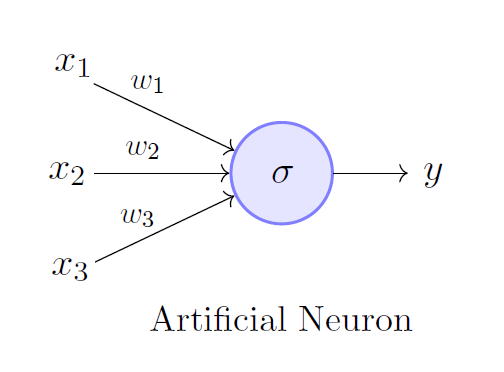
\includegraphics[width=\columnwidth]{04-Figuras/fig}
\caption{Estrutura de um neurônio artificial}

\label{figura:arquitetura}

\end{figure}
De forma geral uma rede neural é constituída de unidades simples de processamento denominadas de neurônios e ligações massivas entre essas unidades.[5]
Mais a frente nessa seção será detalhado a constituição de Redes MLP e anociassociativos competitivas


\subsection{Perceptrom de Multiplas Camadas}

A rede perceptron de múltiplas camadas como o próprio nome indica apresenta várias camadas em sua estrutura,tendo como composição mínima uma camada de entrada, uma camada de saída e uma camada intermediária. Segundo o modelo descrito por [5], essas camadas são ligadas por sinapses com pesos(\textit{pij}) intrínsecos, assim compondo uma rede vasta de interconexões regidas por pesos e funções de ativação.
\begin{figure}[H]

\centering % para centralizarmos a figura
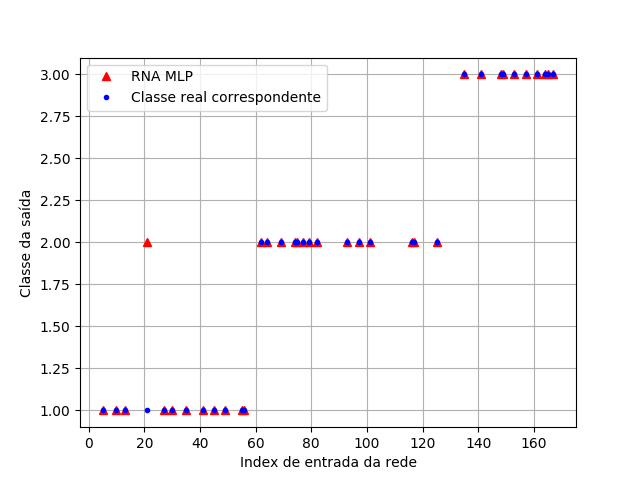
\includegraphics[width=\columnwidth]{04-Figuras/MLP}
\caption{Estrutura de um neurônio artificial}

\label{figura:Arquitetura de uma rede MLP}

\end{figure}

O aprendizado da MLP consiste em 2 passos, o passo direto e o passo inverso. O passo direto ou \textit{forward pass} consiste em passar as entradas pela rede, assim aplicando os pesos associados as sinapses, e obtendo assim a saída. O segundo passo consiste na retropropagação do erro, é calculado o gradiente da função de perda na camada de saída, posteriormente esse gradiente é utilizado para aplicar recursivamente a regra da cadeia para atualizar os pesos de toda a rede.
Esse algorítimo é chamado de \textit{backpropagation}[1].

\subsection{Redes Autoassociativas competitivas}
Redes neurais do tipo autoassociativas ou \textit{autoencoders} baseiam-se em MPL que apresentam o mesmo número de neurônios na camada de entrada e na camada de saída, a camada intermediária apresenta um número inferior de neuronios em relação as outras duas camadas. 

A estrutura da camada de entrada juntamente com a camada intermediária funcionam como um encoder, também chamada de gargalo, comprime a informação inserida na entrada. 

A estrutura de saída juntamente com a camada intermediária funciona como um decoder, descomprimindo a informação obtida da camada intermediária.Dessa maneira, a rede  tenta recriar os dados que foram inseridos na entrada[6].
\begin{figure}[H]

\centering % para centralizarmos a figura
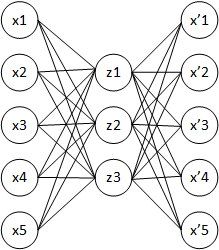
\includegraphics{04-Figuras/autoencoder}
\caption{Estrutura de rede autoencoder}

\label{figura:arquitetura}

\end{figure}

A estrutura competitiva baseia-se em criar e treinar um numero de redes autoencoders igual ao número de classes do problema de classificação, de forma a criar redes especializadas em recriar os dados de entrada de inseridos para cada classe. Dessa forma, as redes treinadas para uma dada classe irão apresentar um erro médio quadrático menor ao serem inseridos dados da classe a qual foram treinadas.

Após o treinamento essas redes são colocadas lado a lado, recebendo as mesmas entradas e tentando recria-las. Mede-se o erro quadrático médio de cada rede para cada índice de entrada, os valores de erro são avaliados e infere-se a classe de saída correspondente a rede que apresentou o menor erro na recriação dos dados de entrada[6].Dessa maneira as redes competem entre si para assim gerar um valor de classe na saída.


%=================================================================================================
\section{Banco de Dados}

A base de banco de dados de vinho selecionada para a produção desse artigo foram resultados de uma análise química de vinhos cultivados na mesma região da Itália,mas derivados de três diferentes cultivares[2].

Os atributos de entrada da rede são Álcool, Acido málico, Cinzas,Alcalinidade das cinzas , Magnésio,Fenóis totais,Flavonoides,Fenóis não flavonoides,Proantocianidinas,Intensidade da cor, tonalidade,OD280 / OD315 de vinhos diluídos e Prolina.

A base de dados foi organizada de forma que cada grupo de 13 variável tem um índex associado e uma classe correspondente.

\begin{table}[H]
\centering
\caption{Distribuição da base de dados}
\begin{tabular}{ccccc}
\hline

\multicolumn{1}{l}{Faixa de Index} & \multicolumn{1}{l}{Classe correspondente} \\ \hline
\textit{0-58}                      & 1                                         \\
58-129                             & 2                                         \\
131-77                             & 3                                         \\ \hline
\end{tabular}%

\label{tabela:baseDados}

\end{table}


 A divisão da base de dados em dados de treino, validação e teste foi realizada com a biblioteca Scikit[7], a qual randomiza a seleção de índex para a divisão do banco de dados em dada proporção previamente programada. A proporção utilizada para a divisão consta na Tabela 2.

\begin{table}[H]
\centering
\caption{Divisão da base de dados}
\resizebox{\columnwidth}{!}{%
\begin{tabular}{cccccccc}
\hline
Distribuição dos dados & \multicolumn{2}{c}{\begin{tabular}[c]{@{}c@{}}Classe 1\\ n        \%\end{tabular}} & \multicolumn{2}{c}{\begin{tabular}[c]{@{}c@{}}Classe 2\\ n        \%\end{tabular}} & \multicolumn{2}{c}{\begin{tabular}[c]{@{}c@{}}Classe 3\\ n        \%\end{tabular}} & Total de Dados \\ \hline
Treino & 35 & 60\% & 44 & 60\% & 27 & 60\% & 106 \\
Validação & 12 & 20\% & 14 & 20\% & 10 & 20\% & 36 \\
Teste & 12 & 20\% & 14 & 20\% & 10 & 20\% & 36 \\ \hline
\end{tabular}
}
\end{table}

 
%=================================================================================================
\section{Desenvolvimento da Rede MLP}
A rede MLP foi desenvolvida em Python[3] com o auxilio da bibliotecas Keras[4].A divisão de dados em treino validação e teste foi seguido como está proposto na Tabela 2, e apesar de que a escolha dos índex de conjunto de entradas é feito de forma randômica, foi fixado duma \textit{seed} na biblioteca Scikit[7], de forma a sempre ser executada a mesma divisão de dados.

A estrutura da rede apresenta 3 camadas, na camada de entrada exite 13 neurônios para receber os dados, a camada de saída dispõe de apenas 1 neurônio. Para definir o numero optimo de neurônios na camada intermediária foi realizado um levantamento da acurácia com relação a esse numero.

\begin{figure}[H]
\centering % para centralizarmos a figura
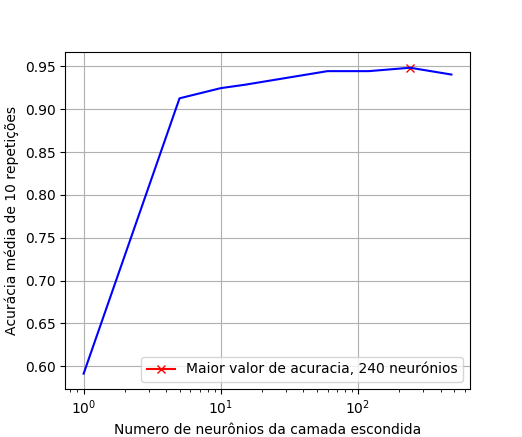
\includegraphics[width=\columnwidth]{04-Figuras/acuracia}
\caption{Acurácia vs Nº de neurônios na camada escondida}
\label{figura:acuracia}
\end{figure}

Depois de definido o número de neurônios da camada escondida, os dados utilizados no treino validação e  teste foram normalizados, de forma que cada coluna dos 13 atributos foi duvidida pelo maior número da coluna.

A função de ativação da camada escondida escolhida foi \textit{sigmoid},a função de ativação da camada de saída foi linear, a escolha das funções foi feita depois de vários testes de desempenho relacionando o erro com a função de ativação escolhida.

A saída da rede foi arredondada para o inteiro mais próximo, por conta que o este tratava-se de um número fracionário.Dessa forma, após arredondar o valor de saída se enquadra em alguma das 3 classes presentes no banco de dados.

\section{Desenvolvimento da Rede Autoencoder competitiva}
Assim como a Rede MLP, a autoencoder competitiva foi deselvolvida utilizando os mesmo software e bibliotecas.A divisão dos dados de entrada em treino validação e teste ocorreu de forma idêntica a rede MLP construida anteriormente.

Feito a divisão de dados de treino de todas as 3 classes, essa foram criadas 3 MLP conectadas de forma competitiva[6]. Essas redes contavam com 13 neurônios na camada inicial e na camada de saída, na camada intermediária foi executado a análise do número de neurônios versus a acurácia total da rede competitiva para descobrir o valor ideal de neurônios na camada intermediária.

\begin{table}[H]
\centering
\caption{Distribuição da base de dados}
\begin{tabular}{cc}
\hline
\begin{tabular}[c]{@{}c@{}}Nº de neurónios na \\ \\ camada escondida\end{tabular} & \begin{tabular}[c]{@{}c@{}}Acurácia média \% \\ \\ de 10 repetições\end{tabular} \\ \hline
1 & 94.44444444 \\
4 & 100 \\
8 & 91.11111111 \\
12 & 69.16666667 \\ \hline
\end{tabular}

\label{tabela:baseDados}

\end{table}


A função de ativação escolhida visando a maior acurácia da rede foi linear tanto na camada escondida quanto na camada de saída.			%-> Desenvolvimento
\section{Resultados}
Após Realizar o treinamento das 2 estruturas de redes propostas, as redes foram colocadas a prova a fim de avaliar seus resultados com os mesmos dados de treino validação e teste, conforme exposto na seção 3 sobre o banco de dados.

\subsection{Resultados MLP}
Depois de selecionado o número ideal para teste dessa estrutura de RNA, foi executado a resposta da rede tendo-se como base dados de teste das 3 classes do banco de dados.
\begin{figure}[H]
\centering % para centralizarmos a figura
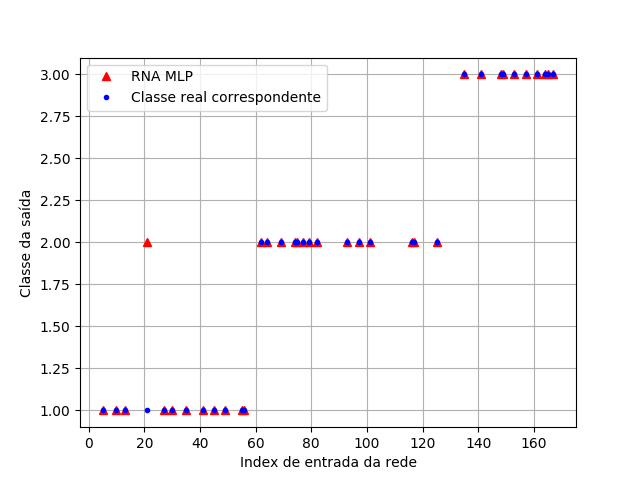
\includegraphics[width=\columnwidth]{04-Figuras/MLP}
\caption{Resposta da rede MLP}
\label{figura:acuracia}
\end{figure}
Realizado 10 repetições de treino validação e teste da rede com os mesmos dados, a percentagem de acerto da rede atingiu a marca de 95.27777778\%.
\subsection{Resultados RNA autoassociativa competitiva}
Feito a análise do melhor número de neurônios na camada escondida para a rede autoassociativa competitiva, cada RNA presente nessa estrutura apresentou um comportamento de erro quadrático médio diferente ao receber dados de teste das 3 classes de vinho presentes no banco de dados.
\begin{figure}[H]
\centering % para centralizarmos a figura
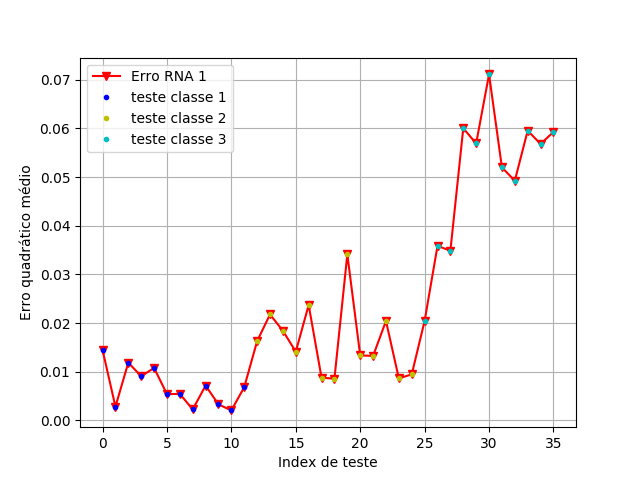
\includegraphics[width=\columnwidth]{04-Figuras/Erro_classe1_auto}
\caption{Erro da Rede 1 exposta os dados de treino}
\label{figura:acuracia}
\end{figure}
\begin{figure}[H]
\centering % para centralizarmos a figura
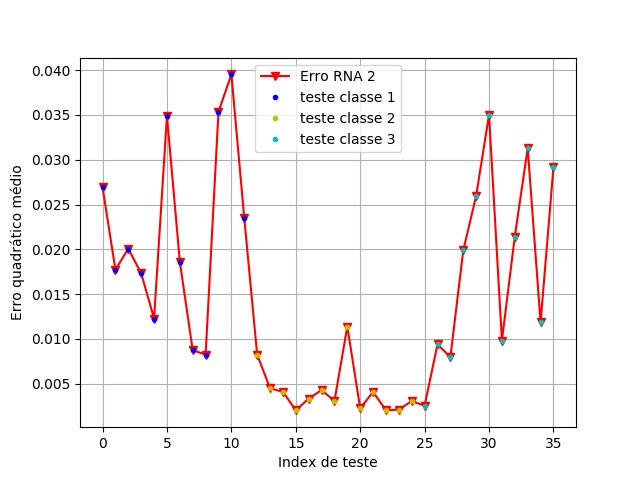
\includegraphics[width=\columnwidth]{04-Figuras/Erro_classe2_auto}
\caption{Erro da Rede 2 exposta os dados de treino}
\label{figura:acuracia}
\end{figure}
\begin{figure}[H]
\centering % para centralizarmos a figura
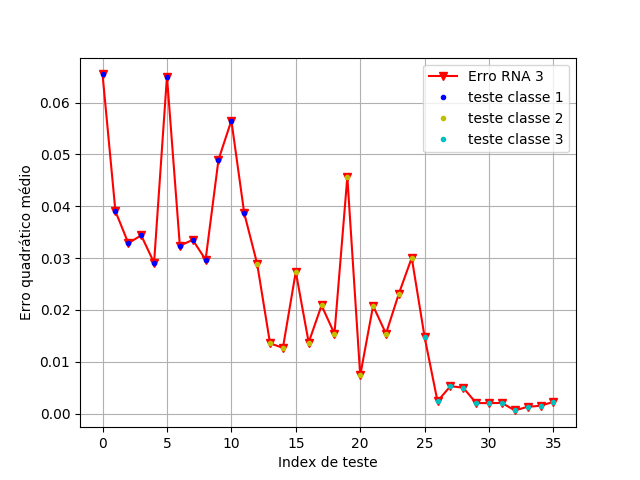
\includegraphics[width=\columnwidth]{04-Figuras/Erro_classe3_auto}
\caption{Erro da Rede 3 exposta os dados de treino}
\label{figura:acuracia}
\end{figure}
Nota-se que a Rede 1, Rede 2 e Rede 3 foram treinadas com bases de dados respectivamente da classe 1,2 e 3.

A saída dessa estrutura de rede se beneficiou do comportamento do erro quadrático médio demonstrado acima, apresentando uma marca de 100\% de acerto médio em 10 repetições de treino validação e teste,  utilizando os mesmos dados de entrada.
\begin{figure}[H]
\centering % para centralizarmos a figura
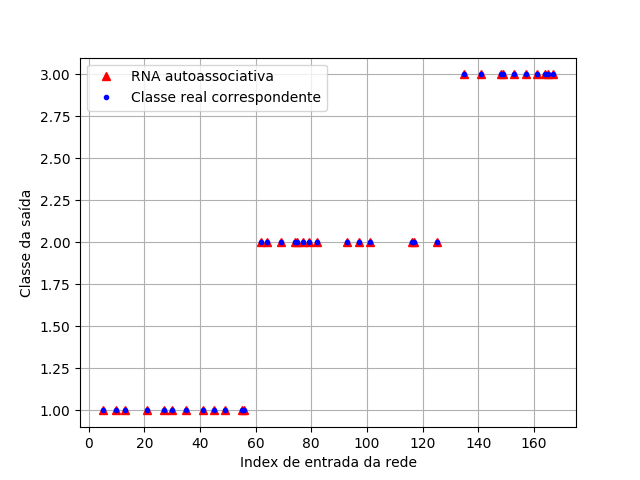
\includegraphics[width=\columnwidth]{04-Figuras/auto_mlp_out}
\caption{Saída da Rede Autoassociativa Competitiva}
\label{figura:acuracia}
\end{figure}
\subsection{Comparativo do desempenho}
Após realizados os testes de desempenho das 2 estruturas,o comparativo de desempenho de ambas foi disposto na Tabela 4.
\begin{table}[H]
\centering
\caption{Comparativo de Desempenho}
\resizebox{\columnwidth}{!}{%
\begin{tabular}{cccc}
\hline
Estrutura da RNA & \begin{tabular}[c]{@{}c@{}}Acurácia média \% \\ \\ de 10 repetições\end{tabular} & Tempo de execução(s) & \begin{tabular}[c]{@{}c@{}}Nº de Épocas\\ \\ utilizadas\\  no treinamento\end{tabular} \\ \hline
MLP & 95.277778 & 3.908075 & 400 \\
\begin{tabular}[c]{@{}c@{}}Autoassociativa \\ \\ competitiva\end{tabular} & 100 & 8.684611 & \begin{tabular}[c]{@{}c@{}}3000 p/ \\ \\ cada rede\end{tabular} \\ \hline
\end{tabular}
}
\label{tabela:baseDados}

\end{table}


Com base nos dados dispostos na Tabela 4, é possível afirmar que a Rede autoassociativa apresentou a marca impecável de 100\% de acerto, devido ao comportamento das redes associadas, de forma que cada rede treinada com dados de apenas 1 classe desempenhava um papel de filtro com relação aos dados das outras classes. De forma que uma rede autoencoder que foi treinada apenas com dados de 1 classe apresentava erro quadrático médio menor quando comparado-se com as outras redes, assim, quando realizado a competição entre as 3 redes treinadas, a classe de saída era escolhida com uma maior acurácia quando comparado-se com o processo de escolha da de apenas uma MLP.					%-> Resultados
\section{Conclusão}

\subsection{Discussão}

Ambas estruturas RNA abordadas nesse artigo apresentaram um desempenho bastante satisfatório, com destaque da Rede autoassociativa competitiva que apresentou 100\% de acerto, uma melhora de de quase 5\% comparado com a estrutura MLP padrão. Para tanto, a rede \textit{autoencoders}  competitiva também apresentou um custo computacional mais elevado, com a utilização de 3000 épocas no treinamento e validação de cada 1 das 3 RNA \textit{autoencoders}.

Dessa forma, para treinar redes dedicadas para cada classe, e nesse processo melhorar o desempenho de classificação a rede autocompetitiva foi mais custosa computacionalmente que a MLP padrão.


\subsection{Conclusão}

Com base no problema de classificação proposto, a rede autoassociativa competitiva apresentou um melhor desempenho na classificação dos tipos de vinho que a rede MLP padrão, com a ressalva do tempo de execução e maior número de épocas de treino validação e teste, o que indica que para outras aplicações na qual há uma maior necessidade em relação a rapidez de treino, ou em aplicações na qual não se dispõe de muito poder computacional, como aplicações em sistemas embarcados, a MLP padrão pode-se apresentar como uma solução melhor.

Tendo-se em vista também a quantidades de index de conjunto de dados do banco de dados analisados, é possível afirmar que o uso de um banco de dados maior poderia acarretar ressaltando o resultado obtido na análise desse artigo.
		%-> Considerações Finais


% ELEMENTOS PÓS-TEXTUAIS =========================================================================

% use section* for acknowledgment
\section*{Acknowledgment}
			%-> Agradecimentos

					%-> Anexo
%=================================================================================================
%=							       		    REFERÊNCIAS											 =
%=================================================================================================


\section{Referências Bibliográficas}
\bibliography{Bibliografia.bib}
			%-> Referências


%=================================================================================================

\end{document}